\documentclass[10pt,a4paper]{article}
\usepackage[utf8]{inputenc}

\usepackage[margin=1.2in]{geometry}

\usepackage{slnwong}

\usepackage{tikz}
\usetikzlibrary{patterns, decorations.pathmorphing}
\tikzset{
	baseline=(current bounding box.north),
	vertex/.style = {shape=circle, draw, minimum size=4mm, inner sep=0, font=\footnotesize},
	bvertex/.style = {shape=circle, draw, minimum size=1.5mm, inner sep=0, fill=black},
	edge/.style = {-, = latex'},
}
\tikzset{arc/.style = {->, = latex}}
\usepackage{multicol}

\title{
	Getting Started
}
\author{slnwong}
\date{\vspace{-5ex}}


\begin{document}

\maketitle
\tableofcontents
\clearpage

\section{Environments}
\begin{definition}
	This is a definition. Usually we have some \vocab{vocab} as well.
\end{definition}

\begin{defn}[Defn]
	For shorthand, we can use `defn'. We can also name the environment.
\end{defn}

\begin{theorem}
	This is a theorem, or `thm' for short.
\end{theorem}

\begin{proposition}
	This is a proposition, or `prop' for short.
\end{proposition}

\begin{lemma}
	This is a lemma, or `lem' for short.
\end{lemma}

\begin{corollary}
	This is a corollary, or `col` for short.
\end{corollary}

\begin{example}
	This is an example.
\end{example}

\begin{note}
	This is a note.
\end{note}

\begin{note}[Named Note]
	Notes can have names too!
\end{note}

\section{Tikz}
Here is a simple graph with `vertex' nodes.
\begin{center}
	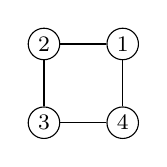
\begin{tikzpicture}
		\node[vertex] (1) at (1,1) {$1$};
		\node[vertex] (2) at (0,1) {$2$};
		\node[vertex] (3) at (0,0) {$3$};
		\node[vertex] (4) at (1,0) {$4$};
		\draw[edge] (1) -- (2);
		\draw[edge] (2) -- (3);
		\draw[edge] (3) -- (4);
		\draw[edge] (4) -- (1);
	\end{tikzpicture}
\end{center}
We can also omit naming the nodes, in which case they are implicitly named $1, 2, \cdots, n$.
\begin{center}
	\begin{tikzpicture}
		\node[vertex] at (1,1) {$1$};
		\node[vertex] at (0,1) {$2$};
		\node[vertex] at (0,0) {$3$};
		\node[vertex] at (1,0) {$4$};
		\draw[edge] (1) -- (2);
		\draw[edge] (2) -- (3);
		\draw[edge] (3) -- (4);
		\draw[edge] (4) -- (1);
	\end{tikzpicture}
\end{center}
We can omit labels for any node.
We can also use `bvertex' if we just want a black dot without labels, or nothing for just an unstyled node with a label
\begin{center}
	\begin{tikzpicture}
		\node[vertex] at (1,1) {};
		\node[vertex] at (0,1) {};
		\node[bvertex] at (0,0) {};
		\node[bvertex] at (1,0) {};
		\node at (0,-1) {a};
		\node at (1,-1) {b};
		\draw[edge] (1) -- (2);
		\draw[edge] (3) -- (4);
	\end{tikzpicture}
\end{center}
We can style (decorate) the edges, e.g. with zigzag lines.
We can also just simply color them.
\begin{center}
	\begin{tikzpicture}
		\node[vertex] at (1,1) {$1$};
		\node[vertex] at (0,1) {$2$};
		\node[vertex] at (0,0) {$3$};
		\node[vertex] at (1,0) {$4$};
		% not sure whats the difference here :/
		% \draw[WildStrawberry] (1) edge[decorate, decoration={zigzag, segment length=4pt}] (2);
		\draw (1) edge[decorate, decoration={zigzag, segment length=4pt}, WildStrawberry] (2);
		\draw[edge, WildStrawberry] (3) -- (4);
	\end{tikzpicture}
\end{center}
We can put labels outside of the node as well.
\begin{center}
	\begin{tikzpicture}
		\node[vertex, label={above:$\textcolor{WildStrawberry}{\frac{1}{4}}$}] at (1,1) {$1$};
		\node[vertex, label={left:$\frac{2}{4}$}] at (0,1) {$2$};
		\node[vertex, label={below:$\frac{3}{4}$}] at (0,0) {$3$};
		\node[vertex, label={right:$\frac{4}{4}$}] at (1,0) {$4$};
		\draw[edge] (1) -- (2);
		\draw[edge] (3) -- (4);
	\end{tikzpicture}
\end{center}
We can also put labels on edges.
\begin{center}
	\begin{tikzpicture}
		\node[vertex] at (1,1) {$1$};
		\node[vertex] at (0,1) {$2$};
		\node[vertex] at (0,0) {$3$};
		\node[vertex] at (1,0) {$4$};
		\draw[edge] (1) -- node[above] {a} (2);
		\draw[edge] (3) -- node[below] {$a$} (4);
	\end{tikzpicture}
\end{center}
Arcs.
\begin{center}
	\begin{tikzpicture}
		\node[vertex] at (1,1) {$1$};
		\node[vertex] at (0,1) {$2$};
		\node[vertex] at (0,0) {$3$};
		\node[vertex] at (1,0) {$4$};
		\draw[arc] (1) -- (2);
		\draw[arc] (3) -- (4);
	\end{tikzpicture}
\end{center}

\section{Math}
Here is an optimization problem.
\[
	\begin{array}{rrclrr}
		\min & \multicolumn{3}{l}{
		w^T x
		} & & (P) \\
		\text{s.t.}
		  & x(\delta(\bar{v})) - x(\delta(v)) & = & b_v & \forall v \in N \\
		& x & \geq & \bm{0}
	\end{array}
\]
% Picture
% \begin{center}
% 	\includegraphics[width=1\textwidth]{image.png}
% \end{center}

\printindex
\end{document}